\subsection{ASL-Phono}
\label{sec:metodologia-datasets-phono}

O ASL-Phono é um \textit{dataset} que introduz uma nova representação baseada na linguística da língua de sinais, a qual descreve os sinais do \acrshort{asllvd} em termos de seus atributos fonológicos. Para computá-los, foram utilizadas as coordenadas 3D fornecidas pelo ASL-Skeleton3D, o que nos forneceu 9.747 amostras e cerca de 2.650 sinais para novo \textit{dataset}.

Como trata-se de uma versão inicial da representação proposta, optamos por selecionar um subconjunto de quatro parâmetros fonológicos dentre aqueles discutidos na \autoref{sec:linguistica-fonologia}, os quais podem ser expandidos em incrementos futuros desta pesquisa. Esses parâmetros incluem a configuração de mão, o movimento da mão, a orientação da palma e uma expressão não-manual refente à abertura da boca, conforme discutiremos a seguir:

\begin{enumerate}
    \item \textbf{Configuração de mão}: refere-se à configurações das mãos do sinalizador durante a articulação dos sinais.
    O \acrshort{asllvd} fornece a configuração de mão inicial e final para cada um de seus sinais, a qual é definida dentre 88 opções apresentadas pelo \acrfull{asllrp}\footnote{Disponível em \url{http://www.bu.edu/asllrp}} \cite{neidle-2020-asllrp}.

    Utilizamos essa informação como base para computar as configurações de mãos no ASL-Phono, mas tivemos que adotar um passo extra para que pudéssemos atribuir configurações a todos os frames das amostras a partir dessas duas únicas providas. Nesse caso, dividimos os frames em duas metades: a primeira, contendo os frames iniciais do sinal, recebeu a configuração de mão inicial provida pelo \acrshort{asllvd}; a segunda, referente aos frames restantes finais, recebeu a configuração final provida.

    % -----
    \item \textbf{Orientação}: refere-se à direção para qual as palmas das mãos apontam durante a articulação dos sinais.
    Para calculá-la, utilizamos um pouco de álgebra linear e exploramos a relação das mãos para com o espaço tridimensional em que suas coordenadas estão representadas \cite{anton-2013-algebra}.

    Para isso, primeiro assumimos cada palma como sendo um plano que atravessa as coordenadas estimadas para as mãos (vide \autoref{subfig:palm-orientation}). A partir disso, selecionamos três coordenadas para descrever este plano: \(W\), que corresponde à coordenada do pulso; \(L\), localizada na base do dedo mínimo; e \(I\), localizada na base do dedo indicador.

    \begin{figure}[ht!]
        \centering
        \caption{
            \textmd{As coordenadas \(W\), \(L\) e \(I\) e os vetores auxiliares são utilizados para obter a normal \(\protect \overrightarrow{n}\) da palma da mão~(\subref{subfig:palm-orientation}).
            A direção da palma \(O_{palm}\) é então calculada a partir de \(\protect \overrightarrow{n}\) e descrita dentre um conjunto de direções possíveis~(\subref{ subfig:palm-directions}).}
        }
        \subcaptionbox{\label{subfig:palm-orientation}}{
            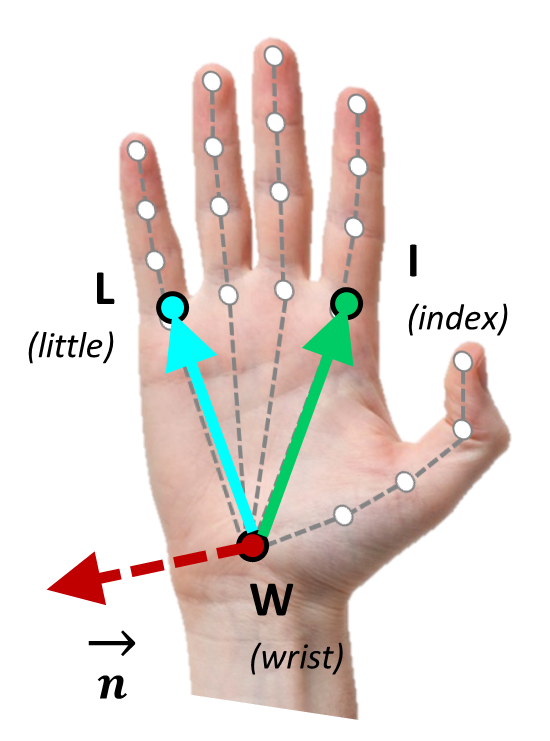
\includegraphics[height=4cm]{capitulos/metodologia/imagens/palm_orientation_algebra}
        }%
        \hspace{1cm}
        \subcaptionbox{\label{ subfig:palm-directions}}{
            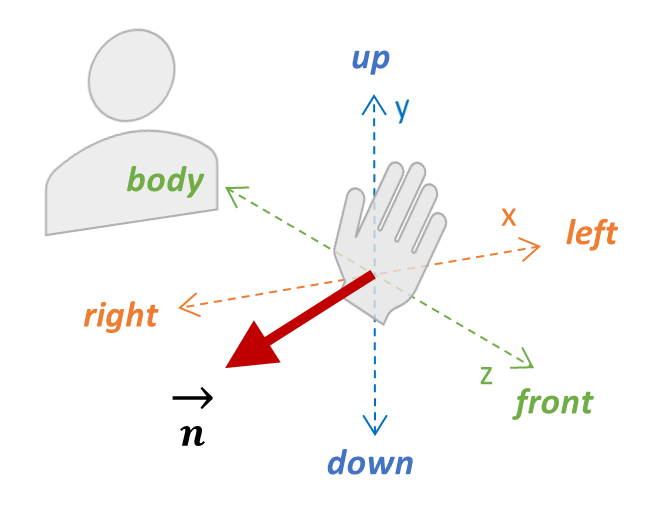
\includegraphics[height=4cm]{capitulos/metodologia/imagens/hand_orientations}
        }%
        \nomefonte{}
        \label{fig:palm-orientation-directions}
    \end{figure}

    Por meio dessas coordenadas, é possível estabelecer dois vetores para descrever o plano da palma (vide \autoref{subfig:palm-orientation}): \(\overrightarrow{WL}\), indicado pela seta azul e \(\overrightarrow{WI}\), indicado pela seta verde. Através deles, é possível estabelecer o vetor normal \(\overrightarrow{n}\) perpendicular ao plano da palma, que é indicado pela seta vermelha tracejada, e calculado conforme \autoref{eqn:normal-palm-left} (para a mão esquerda) e \autoref{eqn:normal-palm-right} (para a mão direita):

    % Palm orientation:
    \begin{equation}
        \label{eqn:normal-palm-left}
        \overrightarrow{n}_{left} = \overrightarrow{WI} \times \overrightarrow{WL}
    \end{equation}

    \begin{equation}
        \label{eqn:normal-palm-right}
        \overrightarrow{n}_{right} = \overrightarrow{WL} \times \overrightarrow{WI}
    \end{equation}


    Finalmente, ao avaliar os valores dos eixos \(x\), \(y\) e \(z\) da normal \(\overrightarrow{n}\), é possível definir a orientação da palma \(O_{palm}\) como sendo a combinação de até três direções, cujas opções são: \textit{right} (direita), \textit{left} (esquerda), \textit{up} (para cima), \textit{down} (para baixo), \textit{body} (para o corpo) ou \textit{front} (para frente).
    Por exemplo, ``\textit{right\_down}'' e ``\textit{left\_up\_body}'' seriam orientações válidas. Essa avaliação é realizada conforme \autoref{eqn:palm-orientation-directions}:
    
    % Directions
    \begin{equation}
        \label{eqn:palm-orientation-directions}
        O_{palm} =
        \begin{cases}
            right & \text{if $\overrightarrow{n}_x < {-k}$ } \\
            left  & \text{if $\overrightarrow{n}_x > {k}$ }  \\
            up    & \text{if $\overrightarrow{n}_y < {-k}$ } \\
            down  & \text{if $\overrightarrow{n}_y > {k}$ }  \\
            body  & \text{if $\overrightarrow{n}_z < {-k}$ } \\
            front & \text{if $\overrightarrow{n}_z > {k}$ }  \\
        \end{cases}
    \end{equation}

    Onde o limiar \(k\) é definido empiricamente como 0,30 para filtrar variações pouco significativas em \(\overrightarrow{n}\). Observe na \autoref{ subfig:palm-directions} como essa operação é aplicada no espaço tridimensional à frente do sinalizador.


    % -----
    \item \textbf{Movimento}: descreve o deslocamento realizado pelas mãos na articulação do sinal.
    De forma semelhante ao que fizemos para a orientação da palma, aqui também analisaremos coordenadas das mãos para determinar sua trajetória no espaço.

    Para isso, utilizaremos a coordenada \(M\) como ponto de referência para as mãos, a qual está localizada na base do dedo médio (vide \autoref{fig:hand-movement-directions}). Com base nela, calcularemos o deslocamento ocorrido entre os frames anterior (tempo \(t-1\)) e atual (tempo \(t\)) para determinar o vetor de movimento \(\overrightarrow{m}\) (indicado pela seta vermelha tracejada), conforme \autoref{eqn:hand-movement}:
    
    % Movement of the hands:
    \begin{equation}
        \label{eqn:hand-movement}
        \overrightarrow{m} = M_{t} - M_{t-1}
    \end{equation}

    \begin{figure}[ht!]
        \centering
        \caption{
            \textmd{O vetor de movimento \(\protect \overrightarrow{m}\) é calculado pela trajetória da coordenada \(M\) entre os frames anterior (\(t-1\)) e atual (\(t\))~(\subref{subfig:hand-movement}).
            O movimento da mão \(V_{hand}\) é então obtido a partir de \(\protect \overrightarrow{m}\) e descrito dentre um conjunto de direções possíveis~(\subref{subfig:hand-directions}).}
        }
        \subcaptionbox{\label{subfig:hand-movement}}{
            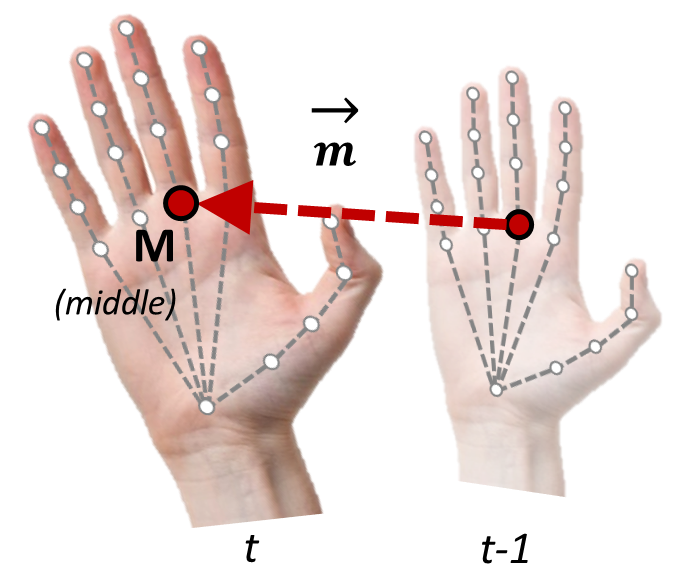
\includegraphics[height=4cm]{capitulos/metodologia/imagens/hand_movement}
        }%
        \hspace{1cm}
        \subcaptionbox{\label{subfig:hand-directions}}{
            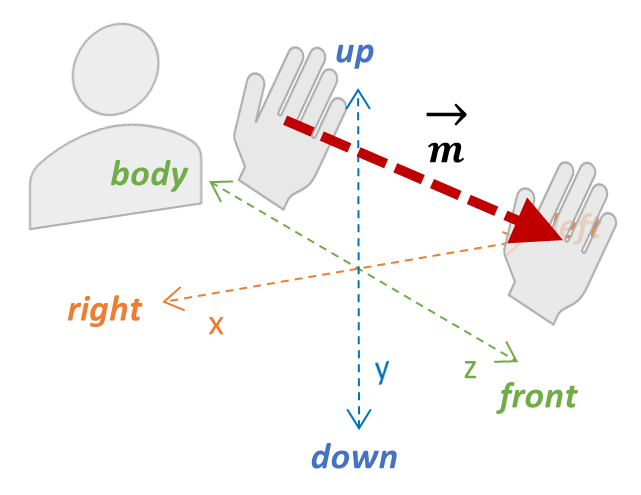
\includegraphics[height=4cm]{capitulos/metodologia/imagens/hand_movement_2}
        }%
        \nomefonte{}
        \label{fig:hand-movement-directions}
    \end{figure}


    A partir do vetor \(\overrightarrow{m}\), aplicamos uma operação parecida com a que foi utilizada para a orientação da mão, para definir o movimento da mão \(V_{hand}\) como a combinação de até três direções, cujas opções são: \textit{right} (direita), \textit{left} (esquerda), \textit{up} (para cima), \textit{down} (para baixo), \textit{body} (para o corpo) ou \textit{front} (para frente). Essa operação é detalhada na \autoref{eqn:hand-movement-directions} e a \autoref{subfig:hand-directions} ilustra ela segundo a perspectiva do sinalizador:

    % Directions
    \begin{equation}
    \label{eqn:hand-movement-directions}
        V_{hand} =
            \begin{cases}
                right & \text{if $\overrightarrow{m}_x < {-k}$ }\\
                left  & \text{if $\overrightarrow{m}_x > {k}$ }\\
                up    & \text{if $\overrightarrow{m}_y < {-k}$ }\\
                down  & \text{if $\overrightarrow{m}_y > {k}$ }\\
                body  & \text{if $\overrightarrow{m}_z < {-k}$ }\\
                front & \text{if $\overrightarrow{m}_z > {k}$ }\\
            \end{cases}    
    \end{equation}

    Aqui o limiar \(k\) também foi definido como 0,30 para remover movimentos pouco significantes.


    % -----
    \item \textbf{Expressão não-manual - abertura da boca}: refere-se à abertura da boca, a cada frame, a qual pode prover significado adicional ao sinal.
    Para calculá-lo, nos baseamos no trabalho de \citeonline{ferrario-2000-study-lips}, o qual analisa e propõe algumas medidas antropométricas para os lábios.

    Dentre essas medidas apresentadas, selecionamos a \textit{vermilion height to mouth width} (ou altura dos lábios com relação à largura da boca), visto que ela é capaz de capturar a abertura dos lábios em termos de uma única proporção. A altura dos lábios é dada pela distância \(d\) entre o \textit{labiale superius} \(LS\) e o \textit{labiale inferius} \(LI\), que são as coordenadas mais externas dos lábios superior e inferior. A largura da boca, por sua vez, é a distância \(d\) entre o \textit{cheilion direito} \(CH_r\) e o \textit{cheilion esquerdo} \(CH_l\), que são as coordenadas do lado direito e esquerdo da boca (vide \autoref{fig:mouth-openness}).

    \figura
        {fig:mouth-openness} % Label
        {capitulos/metodologia/imagens/mouth_openness} % Path
        {height=4cm} % Size
        {A abertura da boca foi calculada com base na medida \textit{vermilion height to mouth width} (ou altura dos lábios com relação à largura da boca) apresentada por \cite{ferrario-2000-study-lips}, a qual considera as coordenadas \(LS\), \(LI\), \(CH_r\) e \(CH_l\).} % Caption
        {ferrario-2000-study-lips} % Citation

        
    Sendo assim, a abertura de boca \(P_{mouth}\) pode ser então definida como na \autoref{eqn:mouth-openness}:

    % Abertura da boca:
    \begin{equation}
        \label{eqn:mouth-openness}
        P_{mouth} = \frac{d(LS, LI)}{d(CH_r, CH_l)}
    \end{equation}

\end{enumerate}


% Estatísticas:
Na \autoref{tab:dataset-phono-stats}, podemos observar algumas estatísticas calculadas a partir do ASL-Phono, que nos permitem compreender como as amostras ficaram organizadas no \textit{dataset} após o processamento acima. 
Nela, os números são listados segundo três perspectivas: 

\begin{itemize}
    \item \textit{Dataset} inteiro: contabiliza o número total de amostras, sinais, movimentos distintos, entre outros, para todo o \textit{dataset}. Por exemplo, pode-se ler que o \textit{dataset} possui 9.747 amostras, 2.650 sinais e 26 movimentos para a mão dominante.
    
    \item Por amostra: contém estatísticas de números mínimos, máximos, médios e desvio padrão para os parâmetros computados acima. Por exemplo, lê-se que, em média, as amostras possuem 3,02 frames, sendo que a mais curta contém apenas 1 frame e a mais longa possui 12 frames. De maneira semelhante, as amostras têm em média de 1,94 movimentos e 2,20 orientações de mão distintas para a mão dominante.

    \item Por sinal: contém estatísticas de números mínimos, máximos, médios e desvio padrão para os sinais contidos no \textit{dataset}. Por exemplo, lê-se que cada sinal possui em média de 3,68 amostras, sendo que alguns deles possuem apenas 1 e outros possuem valores atípicos de 59 amostras (a considerar pelo desvio padrão apresentado). Além disso, cada sinal apresenta em média 6,04 movimentos e 5,37 orientações de mão distintas para a mão dominante.
\end{itemize}

% Please add the following required packages to your document preamble:
% \usepackage{multirow}
% \usepackage{graphicx}
% \usepackage[table,xcdraw]{xcolor}
% If you use beamer only pass "xcolor=table" option, i.e. \documentclass[xcolor=table]{beamer}
\begin{table}[]
    \centering
    \caption{Estatísticas calculadas a partir do ASL-Phono, as quais são visualizadas para todo o \textit{dataset} e segundo agrupamentos por amostra e por sinal. (D) refere-se à mão dominante e (ND) refere-se à mão não-dominante.}
    \label{tab:dataset-phono-stats}
    \resizebox{0.9\textwidth}{!}{%
        \begin{tabular}{cr|ccc|ccccccc}
            \hline
            \rowcolor[HTML]{EFEFEF}
                                                                                     &        & \cellcolor[HTML]{EFEFEF}                           & \cellcolor[HTML]{EFEFEF}                         & \cellcolor[HTML]{EFEFEF}                         & \multicolumn{2}{c}{\cellcolor[HTML]{EFEFEF}Movimento} & \multicolumn{2}{c}{\cellcolor[HTML]{EFEFEF}Orientação} & \multicolumn{2}{c}{\cellcolor[HTML]{EFEFEF}Config. mão} & \cellcolor[HTML]{EFEFEF}                                                                                                                       \\
            \rowcolor[HTML]{EFEFEF}
                                                                                     &        & \multirow{-2}{*}{\cellcolor[HTML]{EFEFEF}Amostras} & \multirow{-2}{*}{\cellcolor[HTML]{EFEFEF}Sinais} & \multirow{-2}{*}{\cellcolor[HTML]{EFEFEF}Frames} & (D)                                                   & (ND)                                                   & (D)                                                     & (ND)                     & (D)  & (ND) & \multirow{-2}{*}{\cellcolor[HTML]{EFEFEF}\begin{tabular}[c]{@{}c@{}}Abertura \\ da boca\end{tabular}} \\ \hline
            \begin{tabular}[c]{@{}c@{}}Dataset \\ inteiro\end{tabular}               &        & 9.747                                              & 2.650                                            & -                                                & 26                                                    & 26                                                     & 26                                                      & 26                       & 85   & 78   & -                                                                                                     \\ \hline
                                                                                     & Mín    & -                                                  & -                                                & 1                                                & 0                                                     & 0                                                      & 0                                                       & 0                        & 0    & 0    & 0,01                                                                                                  \\
                                                                                     & Máx    & -                                                  & -                                                & 12                                               & 10                                                    & 8                                                      & 6                                                       & 5                        & 2    & 2    & 2,19                                                                                                  \\
                                                                                     & Média  & -                                                  & -                                                & 3,02                                             & 1,94                                                  & 1,26                                                   & 2,20                                                    & 1,18                     & 1,17 & 0,72 & 0,13                                                                                                  \\
            \multirow{-4}{*}{\begin{tabular}[c]{@{}c@{}}Por \\ amostra\end{tabular}} & Desvio & -                                                  & -                                                & 0,87                                             & 0,83                                                  & 1,15                                                   & 0,79                                                    & 1,07                     & 0,38 & 0,58 & 0,12                                                                                                  \\ \hline
                                                                                     & Mín    & 1                                                  & -                                                & -                                                & 1                                                     & 0                                                      & 1                                                       & 0                        & 1    & 0    & 0,02                                                                                                  \\
                                                                                     & Máx    & 59                                                 & -                                                & -                                                & 24                                                    & 16                                                     & 22                                                      & 14                       & 8    & 8    & 0,99                                                                                                  \\
                                                                                     & Média  & 3,68                                               & -                                                & -                                                & 6,04                                                  & 3,66                                                   & 5,37                                                    & 2,63                     & 1,81 & 1,17 & 0,13                                                                                                  \\
            \multirow{-4}{*}{\begin{tabular}[c]{@{}c@{}}Por \\ sinal\end{tabular}}   & Desvio & 2,67                                               & -                                                & -                                                & 2,93                                                  & 3,18                                                   & 2,29                                                    & 2,35                     & 0,99 & 1,14 & 0,07                                                                                                  \\ \hline
        \end{tabular}%
    }
    \nomefonte{}
\end{table}


% Exemplo de amostra:
As amostras no ASL-Phono possuem uma estrutura semelhante àquela apresentada para o ASL-Skeleton3D. A diferença, no entanto, está na propriedade "frames", que ao invés de listar coordenadas 3D agora inclui os respectivos atributos fonológicos computados para os frames. Cada atributo, por sua vez, contém o seu respectivo valor e pode conter um \textit{score}, que identifica sua acurácia com base na acurácia das coordenadas envolvidas no seu processamento.

\figura
    {fig:sample-json-phono} % Label
    {capitulos/metodologia/imagens/code_phono} % Path
    {width=0.65\linewidth} % Size
    {Exemplo de amostra do ASL-Phono e propriedades fornecidas para ela.} % Caption
    {} % Citation


O \textit{dataset} resultante do processamento acima e o código-fonte utilizado para isso estão disponíveis publicamente na URL listada abaixo\footnote{Disponível em \url{http://www.cin.ufpe.br/~cca5/asl-phono}}.